\section{Estudio sobre la expresividad de las redes neuronales profundas y no profundas}

\begin{frame}{Objetivos}
	\begin{itemize}
		\item Modelizar una \textbf{tarea de aprendizaje automático}.
		\item Modelizar \textbf{dos tipos de arquitecturas} de aprendizaje automático.
		      \begin{itemize}
			      \item Arquitectura \textbf{profunda}.
			      \item Arquitectura \textbf{no profunda} o somera.
		      \end{itemize}
		\item Dar dos resultados para estudiar el fenómeno de \textbf{eficiencia en profundidad} y cómo de frecuentemente ocurre.
	\end{itemize}
\end{frame}

\subsection{Tarea de aprendizaje}
\begin{frame}{Tarea de aprendizaje}

	\begin{itemize}
		\item Buscamos resolver una tarea de \textbf{clasificación de imágenes}.
		\item Representamos las imágenes de entrada como \textbf{parches}, $(\nv{x_1}, \ldots, \nv{x_N})$ con $\nv{x_i} \in \R^S$. Esta representación se utiliza en la práctica \cite{matematicas:vit}.
		\item Clasificamos la imagen de entrada como el valor $y$ para el cual se maximiza la \textbf{función de puntuación} $h_y: \R^S \times \cdots \R^S \to \R$.
		\item Por lo tanto, buscamos aprender $Y$ funciones de puntuación a partir de los datos y las arquitecturas de aprendizaje automático que desarrollemos.
	\end{itemize}

\end{frame}

\begin{frame}{Función de puntuación}

	\begin{itemize}
		\item \textbf{Funciones de representación} $\conjunto{f_d(\nv{x}): \; d \in \N} \subseteq L^2(\R^S)$. El conjunto de funciones será total y linealmente independiente.
		\item Expresamos las combinaciones lineales finitas como:

		      \begin{equation} \label{eq:hipotesis_en_general}
			      h_y(\nv{x_1}, \ldots, \nv{x_N}) \approx \sum_{d_1, \ldots, d_N \in \N} A^y_{d_1, \ldots, d_N} \prod_{i = 1}^N f_{d_i}(\nv{x_i}).
		      \end{equation}
		\item En \cite{matematicas:principal} se justifica empíricamente que al trabajar con imágenes podemos tomar $M=100$ con lo que se verifica:

		      \begin{equation} \label{eq:puntuacion_general}
			      h_y(\nv{x_1}, \ldots, \nv{x_N}) = \sum_{d_1, \ldots, d_N = 1}^{M} \mathcal{A}^y_{d_1, \ldots, d_N} \prod_{i = 1}^N f_{\theta_{d_i}}(\nv{x_i}).
		      \end{equation}
	\end{itemize}

\end{frame}

\subsection{Modelización de las redes no profundas}


\subsection{Modelización de las redes profundas}



\subsection{Modelización de las redes neuronales}
\begin{frame}
	\begin{block}{Teorema de pruebas}
		Este es un teorema de pruebas
	\end{block}
\end{frame}

\subsection{Teoremas centrales}
\begin{frame}
	\begin{block}{Teorema de pruebas}
		Este es un teorema de pruebas
	\end{block}

	\begin{block}{Otro Teorema de pruebas}
		Otro Este es un teorema de pruebas
	\end{block}
\end{frame}

\begin{frame}

	\begin{figure}
		\centering
		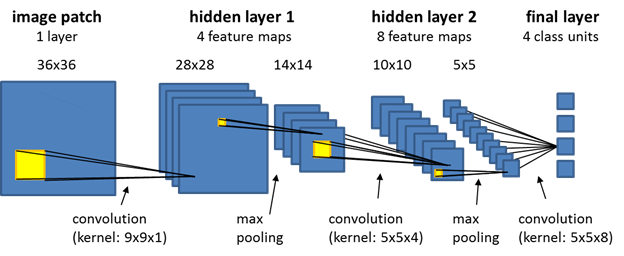
\includegraphics[width=1.0\textwidth]{matematicas/cnn_ejemplo.png}
		\caption{Ejemplo visual de una red convolucional profunda.}
	\end{figure}

\end{frame}

\subsection{Conclusiones}
\begin{frame}
	\begin{itemize}
		\item Primera conclusion
		\item Segunda conclusion
		\item Tercera conclusion
	\end{itemize}
\end{frame}
